\subsection{Interrelación Asesor Curso Académico - Plantilla Entrevista Asesor}

   \begin{description}
      \item[Definición] En esta interrelación se deja constancia de que un
      usuario asesor puede usar plantillas de entrevistas de asesor durante un
      determinado curso académico.

      \begin{itemize}
       \item Un \textit{Asesor Curso Académico} puede utilizar varias
             \textit{Plantilla Entrevista Asesor}.
       \item Una \textit{Plantilla Entrevista Asesor} solamente puede ser
             utilizada por un \textit{Asesor Curso Académico}.
      \end{itemize}

      \item[Características] La interrelación presenta las siguientes
                             características:

         \begin{itemize}
            \item \textbf{Nombre:} AseCA-PEA
            \item \textbf{Tipo de la interrelación:} El tipo de entidad
            Plantilla Entrevista Asesor es débil por identificación respecto al
            tipo de entidad Asesor Curso Académico.
            \item \textbf{Cardinalidad de la interrelación:} 1:N
                  \begin{itemize}
                     \item Asesor Curso Académico: utiliza (0,n)
                     \item Plantilla Entrevista Asesor: utilizada\_por (1,1)
                  \end{itemize}
            \item \textbf{Número de atributos:} Ninguno.
         \end{itemize}

      \item[Diagrama] La figura \ref{diagramaAseCA-PEA} muestra el diagrama de
      la interrelación.

      \item \begin{figure}[!ht]
            \begin{center}
            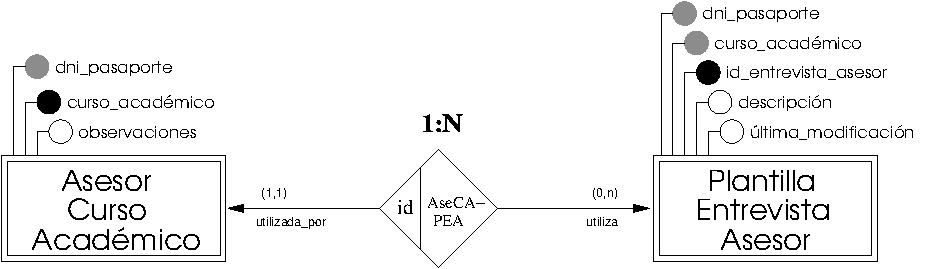
\includegraphics[]{07.Modelo_Entidad-Interrelacion/7.3.Analisis_Interrelaciones/diagramas/AseCA-PEA.pdf}
            \caption{Diagrama de la interrelación AseCA-PEA.}
            \label{diagramaAseCA-PEA}
            \end{center}
         \end{figure}

      \item[Ejemplo práctico del tipo de interrelación]

      \item \begin{center}
            \begin{tabular}{ | r r | }
            \hline
            \multicolumn{2}{ | c | }{\textbf{Tipo de interrelación AseCA-PEA}} \\
            \hline
            \textbf{Asesor Curso Académico} & \\
            dni\_pasaporte & 98765432Z \\
            curso\_académico & 2008 \\
            \hline
            \textbf{Plantilla Entrevista Asesor} & \\
            dni\_pasaporte & 98765432Z \\
            curso\_académico & 2008 \\
            id\_entrevista\_asesor & 36 \\
            \hline
            \end{tabular}
         \end{center}
   \end{description}
